\input{preamble}
\usepackage{cancel}
\usepackage{tikz}
\usetikzlibrary{positioning}
\usetikzlibrary{shapes}

\title{}
\author{Dane Jeon}
\affiliation{Sogang University,\\
35 Baekbeom-ro, Mapo-gu, Seoul 04107, Republic of Korea}
\emailAdd{danetrouveur@gmail.com}
\abstract{In this document, we try to exploit the symmetries that exist in the action and find the whole set of equations of motion of the action up to permutation.}

\begin{document}

\begin{defi}
(Action) In this document, we consider the following integrand whose integral would give the action (notice that we are using a capital $L$ to denote $\mathcal{L}\sqrt{-g}\,d^{4}x$ where $\mathcal{L}$ would be the Lagrangian density that we know. In this document, we call both the ``lagrangian density" exchangeably):
\[L=(R-V)\star 1+L_{KinS}+L_{KinA}+L_{CS}\]
where $V$, $L_{KinS}$, $L_{KinA}$, and $L_{CS}$ are defined as
\[V=-4g^2\sum _{i}(Y_{i}^2+\tilde{Y}_{i}^2)\]
\[L_{KinS}=-\dfrac{1}{2}\sum _{i}\Big((\partial \varphi_{i})^2+e^{2\varphi _{i}}(\partial \chi _{i})^2\Big)\star 1\]

\begin{align*}
L_{KinA}= -\tfrac{1}{2} |W|^{-2} \Big[ 
P_0 \Big(& \tilde{Y}_1^2 \tilde{Y}_2^2 \tilde{Y}_3^2\star  F_1\wedge  F_1 + \tilde{Y}_1^2 Y_2^2 Y_3^2 \star F_2 \wedge  F_2 \\
+& {Y}_1^2 \tilde{Y}_2^2 Y_3^2\star F_3  \wedge  F_3 + Y_1^2 {Y}_2^2 \tilde{Y}_3^2 \star F_4\wedge F_4\Big)\\
+&2P_1 b_2 b_3 \Big(\tilde{Y}_1^2\star  F_1 \wedge F_2 - Y_1^2 \star F_3\wedge F_4\Big) \\
+& 2P_2 b_1 b_3 \Big(\tilde{Y}_2^2\star  F_1 \wedge F_3 - Y_2^2 \star F_2 \wedge F_4\Big) \\
+& 2P_3 b_1 b_2 \Big(\tilde{Y}_3^2 \star F_1\wedge F_4 - Y_3^2\star  F_2 \wedge F_3 \Big) 
\Big]
\end{align*}
\begin{align*}
L_{CS}=-|W|^{-2} \Big[
b_1 b_2 b_3 \Big(& \tilde{Y}_1^2 \tilde{Y}_2^2 \tilde{Y}_3^2 F_1 \wedge F_1 + \tilde{Y}_1^2 {Y}_2^2 Y_3^2 F_2 \wedge F_2 \right. \\
+& {Y}_1^2 \tilde{Y}_2^2 {Y}_3^2 F_3 \wedge F_3 + Y_1^2 {Y}_2^2 \tilde{Y}_3^2 F_4 \wedge F_4 \Big) \\
+& b_1 (P_0 + 2b_2^2 b_3^2)\Big(\tilde{Y}_1^2 F_1 \wedge F_2 - Y_1^2 F_3 \wedge F_4 \Big) \\
+& b_2( P_0 + 2b_1^2 b_3^2)\Big(\tilde{Y}_2^2 F_1 \wedge F_3 - Y_2^2 F_2\wedge F_4 \Big) \\
+& b_3 (P_0 + 2b_1^2 b_2^2)\Big(\tilde{Y}_3^2 F_1 \wedge F_4 - Y_3^2 F_2 \wedge F_3 \Big) 
\Big]
\end{align*}
\end{defi}
\vspace{2ex}
Meanwhile, the implicit functions $Y_{i}^2$, $\tilde{Y}_{i}^2$, and $b_{i}$ are defined as
\[Y_{i}^2=e^{\varphi _{i}}\quad \tilde{Y}_{i}^2=e^{-\varphi _{i}}+\chi _{i}^2e^{\varphi _{i}}\quad b_{i}=\chi _{i}e^{\varphi  _{i}}\]
and additionally,
\begin{align*}
P_{0}&=1+b_1^2+b_2^2+b_3^2&W&=P_0-2i\,b_1b_2b_3\\
P_1&=1-b_1^2+b_2^2+b_3^2&P_2&=1+b_1^2-b_2^2+b_3^2&P_3&=1+b_1^2+b_2^2-b_3^2
\end{align*}
\begin{thm}
(Symmetries in the action) We now investigate the symmetries inside the action to find the number of equation of motions we need to calculate up to permutation. Assuming no symmetry, we have a total of 6 independent fields $\varphi _{i}$ and $\chi_{i}$ (for $i\in \{1,2,3\}$) and 4 gauge fields $A_{j}$  (for $j\in \{1,2,3,4\}$), and one metric field $g_{\mu \nu }$, giving us a total of $6+4+1$ equations.

First notice that $V$ and $L_{KinS}$ are not affected by any permutation of identical fields. It therefore suffices to examine the symmetries in the $L_{KinA}$ and $L_{CS}$ term. By careful observation, we find the following two symmetries among fields, where permutations with the same label are acted strictly together.

\begin{center}
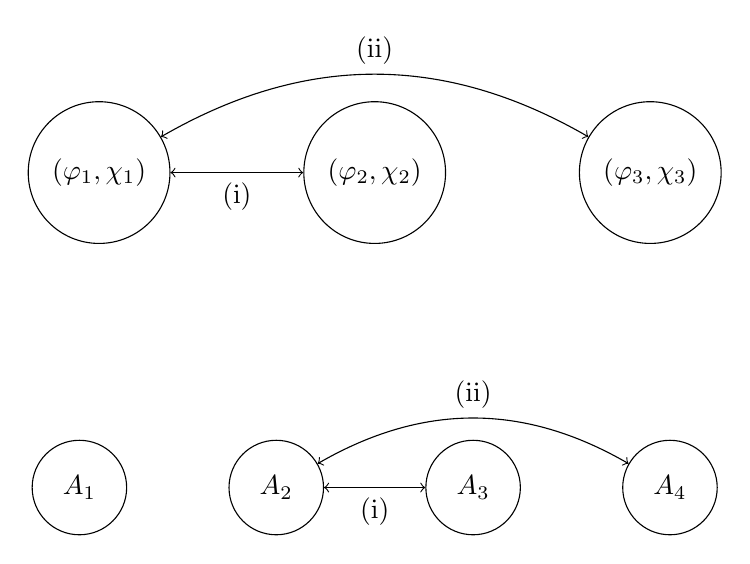
\begin{tikzpicture}[
  pairnode/.style={draw, circle, minimum size=1.8cm, align=center},
  Anode/.style={draw, circle, minimum size=1.2cm, align=center},
  node distance=2.5cm
]

% Top part: (ϕ_i, χ_i) pairs — with circles
\node[pairnode] (set1) at (0,0) {$(\varphi_1,\chi_1)$};
\node[pairnode] (set2) at (3.5,0) {$(\varphi_2,\chi_2)$};
\node[pairnode] (set3) at (7,0) {$(\varphi_3,\chi_3)$};

% Arrows for top
\draw[<->] (set1) -- node[below] {(i)} (set2);
\draw[<->, bend left=30] (set1) to node[above] {(ii)} (set3);

% Bottom part: A_i states — with circles
\node[Anode] (A1) at (-0.25,-4) {$A_1$};
\node[Anode] (A2) at (2.25,-4) {$A_2$};
\node[Anode] (A3) at (4.75,-4) {$A_3$};
\node[Anode] (A4) at (7.25,-4) {$A_4$};

% Arrows for bottom
\draw[<->] (A2) -- node[below] {(i)} (A3);
\draw[<->, bend left=30] (A2) to node[above] {(ii)} (A4);

\end{tikzpicture}
\end{center}
This tells us that we only need to find one equation for each scalar field, two equations from the gauge fields, and one metric field, giving us a total of $1+2+1=5$ equations. 
\end{thm}
\vspace{2ex}
\begin{defi}
(The trunction limit) We define the truncation limit as the following set of limits
\[
\[\begin{cases}
    \phi_1 \to \xi \\
    \chi_1 \to \chi \\
    A_1 \text{ and } A_2 &\to A_3 \\
    A_3 \text{ and } A_4 &\to A_1
\end{cases}\]
\]
While the remaining fields are put to 0. We can additionally impose the following limits such that the equations of motion would reduce to the one in Cassani’s paper.
\[
\left\{
\begin{aligned}
    A_i &\to \frac{1}{\sqrt{2}} A_i \\
    g &\to \frac{1}{2} g
\end{aligned}
\right.
\]

\end{defi}
\vspace{2ex}

\begin{prop}
(Variation with respect to the dilaton field $\varphi  _1$) With the above definitions, our strategy in finding and verifying the equations or motion for the scalar fields are straightforward: 
\begin{itemize}
\item[(i)] We first gather terms that are relevant in the variation process 
\item[(ii)] By simply differentiating the terms in the lagrangian density with respect to the scalar term of interest, we find $\delta L_{KinA}/\delta \varphi_1$ (the term $L_{KinA}$ can be replaced with any term in the Lagrangian density and the field $\varphi_1$ can be replaced with any scalar field)
\item[(iii)] We verify the equations by taking the truncation limit and the Cassani paper conventions defined above, we verify that our scalar field equations are indeed correct.
\end{itemize}
In this document, we only show the implicit versions of the equations of motion, while the entirety is displayed in the mathematica file. 
\[\begin{align*}
\delta _{\varphi_1}S=\int \delta \varphi_1\Big[-4g^2(e^{\varphi _1}&-e^{-\varphi _1}+\chi_1^2e^{\varphi _1})\star 1+d(\star d\varphi_1)\\&-e^{2\varphi_1}d \chi_{1}\wedge \star d \chi_{1}+1 +\dfrac{\delta L_{kinS}}{\delta \varphi_1}+\dfrac{L_{KinA}}{\delta \varphi_1}+\dfrac{\delta L_{CS}}{\delta \varphi_1}\Big]
\end{align*}\]
We therefore have
\[0=-4g^2(e^{\varphi_1}-e^{-\varphi_1}+\chi_1^2e^{\varphi_1})\star 1+d(\star d\varphi_1)-e^{2\varphi_1}d \chi_{1}\wedge \star d \chi_{1}+\dfrac{\delta L_{KinS}}{\delta \varphi_1}+\dfrac{\delta L_{KinA}}{\delta \varphi_1}+\dfrac{\delta L_{CS}}{\delta \varphi_1}\]
\end{prop}
\vspace{2ex}
\begin{prop}
(Variation with respect to the axion field $\chi $) Again, we have the implicit version as
\[\delta_{\chi_1}S=\int \delta \chi_1\Big[-8g^2\chi_1e^{\varphi _1}\star 1-\dfrac{1}{2}d(e^{2\varphi_1}\star d\chi_1)+\dfrac{\delta L_{KinS}}{\delta \chi_1}+\dfrac{\delta L_{KinA}}{\delta \chi_1}+\dfrac{\delta L_{CS}}{\delta \chi_1}\Big]\]
We therefore have
\[0=-8g^2\chi_1e^{\varphi_1}\star 1-\dfrac{1}{2}d(e^{2\varphi_1}\star d\chi_1)+\dfrac{\delta L_{KinS}}{\delta \chi_1}+\dfrac{\delta L_{KinA}}{\delta \chi_1}+\dfrac{\delta L_{CS}}{\delta \chi_1}\]
\end{prop}
\vspace{2ex}
\begin{prop}
(Variation with respect to gauge field $A_1$) For the gauge fields, we preform a straight forward variation and find
\[\delta _{A_1}S=\int \delta_{A_1}(L_{KinS}+L_{KinA}+L_{CS})\]
Resulting in
\[
\begin{align*}
0= d\Big(|W|^{-2}\Big[&-\dfrac{1}{2}P_0\tilde{Y}_{1}^2\tilde{Y}_{2}^2\tilde{Y}_{3}^2\star F_1\\&-P_1b_2b_3\tilde{Y}_{1}^2\star F_2-P_2b_1b_3\tilde{Y}_{2}^2\star F_3-P_3b_1b_2\tilde{Y}_{3}^2\star F_4\\&-b_1b_2b_3\tilde{Y}_{1}^2\tilde{Y}_{2}^2\tilde{Y}_{3}^2\star F_1\\&-b_1(P_0+2b_2^2b_3^2)\tilde{Y}_{1}^2\star F_2-b_2(P_0+2b_1^2b_3^2)\tilde{Y}_{2}^2\star F_3+b_3(P_0+2b_1^2b_2^2)\tilde{Y}_{3}^2\star F_4\Big]\Big)
\end{align*}
\]
\end{prop}
\vspace{2ex}
\begin{prop}
(Variation with respect to gauge field $A_2$)
\[\delta _{A_1}S=\int \delta _{A_1}(L_{KinS}+L_{KinA}+L_{CS})\]
Resulting in
\[
\begin{align*}
0=d\Big(|W|^{-2}\Big[P_0\tilde{Y}_{1}^2Y_{2}^2Y_{3}^2\star F_2+2P_1b_2b_3\tilde{Y}_{1}^2\star F_{1}-2P_{2}b_1b_3Y_{2}^2\star F_{4}-2P_3b_1b_2Y_{3}\star F_3\Big]\Big)
\end{align*}
\]
\end{prop}
\vspace{2ex}
\begin{prop}
(Variation with repsect to metric field $g_{\mu \nu }$) The only terms in the lagrangian density that depend on the metric are $R\star 1$, $L_{KinS}$, and $L_{KinA}$. Before we apply the variation, we first write the relevant terms in component form. 
\[R=g^{\mu \nu }R_{\mu \nu }\qquad \mathcal{L}_{kinS}=-\dfrac{1}{2}g^{\mu \nu }\sum _{i}(\partial _{\mu }\varphi _{i}\partial _{\nu }\varphi  _{i}+e^{2\varphi_{i}}\partial _{\mu }\chi _{i}\partial _{\nu }\chi _{i})\]
\begin{align*}
\mathcal{L}_{KinA}= -\tfrac{1}{8} |W|^{-2} \Big[ 
P_0 \Big(& \tilde{Y}_1^2 \tilde{Y}_2^2 \tilde{Y}_3^2 (F_1)^{\mu\nu}(F_1)_{\mu\nu}
+ \tilde{Y}_1^2 Y_2^2 Y_3^2 (F_2)^{\mu\nu}(F_2)_{\mu\nu} \\
+& {Y}_1^2 \tilde{Y}_2^2 Y_3^2 (F_3)^{\mu\nu}(F_3)_{\mu\nu}
+ Y_1^2 {Y}_2^2 \tilde{Y}_3^2 (F_4)^{\mu\nu}(F_4)_{\mu\nu} \Big)\\
+& 2P_1 b_2 b_3 \Big(\tilde{Y}_1^2 (F_1)^{\mu\nu}(F_2)_{\mu\nu} - Y_1^2 (F_3)^{\mu\nu}(F_4)_{\mu\nu} \Big) \\
+& 2P_2 b_1 b_3 \Big(\tilde{Y}_2^2 (F_1)^{\mu\nu}(F_3)_{\mu\nu} - Y_2^2 (F_2)^{\mu\nu}(F_4)_{\mu\nu} \Big) \\
+& 2P_3 b_1 b_2 \Big(\tilde{Y}_3^2 (F_1)^{\mu\nu}(F_4)_{\mu\nu} - Y_3^2 (F_2)^{\mu\nu}(F_3)_{\mu\nu} \Big) 
\Big]
\end{align*}
where we have omited the volume element $\sqrt{-g}\,d^{4}x$. We know that the Einstein field equation is given as
\[\dfrac{\delta \mathcal{L}}{\delta g^{\mu \nu }}-\dfrac{1}{2}g_{\mu \nu }\mathcal{L}=0\]
which we can compute for our action to be
\begin{align*}
R_{\mu \nu }-\dfrac{1}{2}\sum _{i}(\partial _{\mu }\varphi _{i}&\partial _{\nu }\varphi _{i}+e^{2\varphi _{i}}\partial _{\mu }\chi _{i}\partial _{\nu }\chi _{i})\\
-\frac{1}{4}|W|^{-2} \Big[ P_0 \Big(& \tilde{Y}_1^2 \tilde{Y}_2^2 \tilde{Y}_3^2 (F_1)_{\mu}^{\ \rho}(F_1)_{\nu\rho}
+ \tilde{Y}_1^2 Y_2^2 Y_3^2 (F_2)_{\mu}^{\ \rho}(F_2)_{\nu\rho} \\
+ &{Y}_1^2 \tilde{Y}_2^2 Y_3^2 (F_3)_{\mu}^{\ \rho}(F_3)_{\nu\rho}
+ Y_1^2 {Y}_2^2 \tilde{Y}_3^2 (F_4)_{\mu}^{\ \rho}(F_4)_{\nu\rho} \Big)\\
+& 2P_1 b_2 b_3 \Big(\tilde{Y}_1^2 (F_1)_{\mu}^{\ \rho}(F_2)_{\nu\rho} - Y_1^2 (F_3)_{\mu}^{\ \rho}(F_4)_{\nu\rho} \Big) \\
+& 2P_2 b_1 b_3 \Big(\tilde{Y}_2^2 (F_1)_{\mu}^{\ \rho}(F_3)_{\nu\rho} - Y_2^2 (F_2)_{\mu}^{\ \rho}(F_4)_{\nu\rho} \Big) \\
+& 2P_3 b_1 b_2 \Big(\tilde{Y}_3^2 (F_1)_{\mu}^{\ \rho}(F_4)_{\nu\rho} - Y_3^2 (F_2)_{\mu}^{\ \rho}(F_3)_{\nu\rho} \Big) 
\Big]\\
-\frac{1}{2}g_{\mu\nu}(R-V&+L_{KinS}+L_{KinA}+L_{CS})
\end{align*}
where we have wrote the last term implicitly. 
\end{prop}
\vspace{2ex}
\end{document}
